\documentclass[11pt]{article}

% Basic packages
\usepackage{amsmath}
\usepackage{graphicx}
\usepackage{parskip}
\usepackage[section]{placeins}
\usepackage[capitalise, noabbrev]{cleveref}
\usepackage{csvsimple}
\usepackage{booktabs}
\usepackage[margin=3cm]{geometry}
\usepackage[table,xcdraw]{xcolor}
\usepackage{tikz}
\usetikzlibrary{math,calc,positioning}

\usepackage[backend=biber]{biblatex}
\bibliography{bibliography}

\usepackage{todonotes}

% Set up fonts
\usepackage{fontspec}
\usepackage{unicode-math}
\setmainfont{STIX Two Text}
\setmathfont{STIX Two Math}

\title{FYS-STK4155 - Project1}
\author{Gard, Are, David Andreas Bordvik}
\date{\today}

\begin{document}

\maketitle

\section*{Question 1}
% \subsection*{Introduction}
The main goal for this task is to predict wind power generation in November 2013 using historical data and different types of machine learning methods. The target variable specified for this task is wind power generation, and we are told to use wind speed 10 meters above the ground as our single feature in the input data for the machine learning model.

In machine learning (ML), the main idea is to create a model that can learn to map input data to outputs. The training process of an ML model results in a model that is fitted to memorize patterns within the data while incorporating relationships between different features. This assignment is based on the supervised learning paradigm, a sub-category out of the four main ML categories; supervised learning, unsupervised learning, semi-supervised learning, and reinforcement learning. Supervised learning relies on the model having access to a target variable during training. For this task, we are given the target variable for power production, which is a continuous target variable. Since the target for the training data is numerical and continuous, and the model's outcome is expected to be continuous, we have a regression problem. Furthermore, the assignment expects a comparison of three classical ML models and one deep learning model. Deep learning is regarded as a subset of machine learning. Deep learning utilizes artificial neural networks (ANN) that mimic the human brain through a set of advanced algorithms. 


\subsection*{The problem}
As mentioned in the above, we face a regression problem using supervised learning, both for the deep learning model and the three classical ML approaches. We consider the problem of predicting wind farm power output based on wind speed.
Let $s$ be wind speed\footnote{Units are nowhere specified, but we presume meters per second.}, and let $p$ be power output\footnote{In watts, but normalised by some unknown amount.}. In ML we assume that there is some unknown function $f$ such that
\begin{equation*}
  p = f(s).
\end{equation*}
We have access to training data in the form of a number of observations $(p_i, s_i)$ such that $p_i = f(s_i)$.
Our task is to use the training data to find an approximation $\hat{f}$ of $f$.
The approximation enables us to estimate $p = f(s)$ by $\hat{p} = \hat{f}(s)$ for previously unseen values of $s$.
A good approximation $\hat{f}$ should give small differences between $p = f(s)$ and $\hat{p} = \hat{f}(s)$.
We use the root-mean-square error (RMSE) to compute the difference between $f$ and $\hat{f}$ over a set of testing data; measurements for November 2013 in our case.
Let $(p_i, s_i)$ for $i \in N$ be test data for November (which was not used as training data for $\hat{f}$).
Then the RMSE between $\hat{f}$ and $f$ is defined as
\begin{equation*}
  \sqrt{\frac{1}{|N|} \sum_{i \in N} \left(\hat{f}(s_i) - p_i\right)^2}.
\end{equation*}

Additionally we want to compare different approaches for predicting $f$.
Some of the approaches (e.g.\ linear regression) give a closed-form expression for $\hat{f}$ while others (e.g.\ nearest-neighbour, neural networks) result in algorithms for computing $\hat{f}$.
We evaluate the effectiveness of each model using the RMSE as discussed above; closer to $0$ is better.
For the artificial neural network model in particular, we also evaluate whether the model may have over-fitted the training data.

% During training, we have access to the true target variable $p$. Performing inference using a trained model on new previously unseen data, the true target variable $p$ is no longer known. However, we can assume that the model predicts $\hat{p}$ not too far from the theoretical true value of the unknown $p$. Optimally the residual deviance between $\hat{p}$ and $p$ should look similar to what can be achieved performing inference on the data the model has been trained on where the true values for $p$ are known. 

% Furthermore, for the ANN model, the assumption above implies that the model is not overfitted or underfitted to the training data, and that the model has been generalized properly during the training process.


\subsection*{Input data and data analysis}
One of the most important aspects of ML is the quality of the data. For our case, we expect that there is a relationship between wind speed $s$ and the actual generated power $p$, given by $f$. 
% The input data must therefore incorporate information influencing the outcome such that the model can learn their relationship. 
However, it's highly likely that other factors besides wind speed at 10m also affect the amount of generated power.
Therefore, we don't expect a ``perfect'' relationship between wind speed and generated power.
Specifically, for any function $f$ depending only on wind speed, the generated power $p$ with a wind speed of $s$ is \emph{close} to $f(s)$, but not always exactly equal.
In other words, even the unknown function $f$ which we want to approximate probably has a non-zero RMSE on the testing data.
This also makes it unlikely for any estimation $\hat{f}$ to achieve a RMSE very close to 0.

The training data we use, contained in the \texttt{TrainData.csv} file, consists of time series data including measurements of wind speed $s$ and power output $p$.
The data consists of hourly measurements from 01.01.2012 to 31.10.2013.
In fact, in addition to the wind speed we are also given the wind speed components in the $x$ and $y$ directions, effectively giving us the wind angle.
This is used in the next question.
Additionally, we have all of the above data measured at two different altitudes: 10 meters and 100 meters.
For this assignment, we only use the measurements taken at 10 meters.

To get some quick intuition about the data, consider the correlation matrix between the different columns in \texttt{TrainData.csv}, in \cref{fig:q1-corr-analysis}.
The most important part of the matrix is the POWER row, showing the correlation between this and the other columns.
We can see that there is a good correlation between POWER and WS10 (the wind speed at 10 meters altitude), which is the parameter we are using.
The correlation with WS100, the wind speed at 100 meters altitude, is even higher, suggesting that this would also be a useful parameter.

\begin{figure}
  \centering
  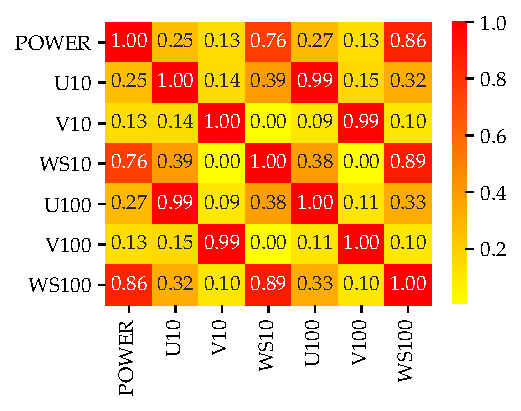
\includegraphics{figures/q1_corr_analysis.pdf}
  \caption{Correlation analysis of columns in \texttt{TrainData.csv}.}
  \label{fig:q1-corr-analysis}
\end{figure}

A high correlation shows a near-linear relationship between two parameters.
This suggests that a linear regression approximation for $f$ should already be quite effective.
Hopefully, more sophisticated methods should give an even higher degree of accuracy than linear regression.

Once we have trained different models on the training data, we use them to predict power output for a new period.
In particular, we have one month (November 2013) of wind speed measurements in the same format as the training data, found in \texttt{WeatherForecastInput.csv}.
Our task is to ``predict'' power output for November 2013 using these measurements.
For testing purposes, we also have the complete measurements (including power data) for November 2013 in \texttt{Solution.csv}.
As previously discussed, we compute the RMSE between the predicted power output and the real data given in \texttt{Solution.csv} in order to evaluate the different models.

\subsection*{Model setup and approach}

We use four different regression models to predict wind power output:
\begin{enumerate}
\item
  Linear regression.
\item
  $k$-Nearest Neighbour (kNN).
\item
  Support Vector Regression (SVR).
\item
  Artificial Neural Network (ANN).
\end{enumerate}

The application of these models is mostly straight-forward, and we refer directly to the attached code for implementation details.
However, for some of the models there are hyperparameters and other choices to discuss.
Short of a rigorous hyperparameter optimisation such as a grid-search, finding the right hyperparameters for particular problems usually involves some experimentation.
In our case, informal experimentation is sufficient as we don't have to deal with many hyperparameters.

There are no hyperparameters for linear regression.

For the $k$-Nearest Neighbour model, we need to choose a value for $k$.
Because we have relatively large amount of training data ($\approx 16000$ points) within a relatively small interval (wind speeds between 0 and 15), we chose a rather large value for $k$.
After some experimentation, the model seems quite insensitive to the value of $k$ in the order of magnitude $[300, 3000]$; we chose $k=1000$.

We use a Support Vector Regression model using the kernel trick, with the Radial Basis Function (RBF) as a kernel function.
This is a standard, flexible kernel function which allows us to fit non-linear data.
Apart from the kernel function, we need to choose the regularization parameter $C$ and the allowed error $\epsilon$.
The parameter $\epsilon$ determines the width of the band around the predicted regression within which the loss function for training data is set to $0$.
Data outside the $\epsilon$-wide band is weighed proportional to $C$ in the loss function (the other component in the loss function being the norm of the vector $\mathbf{w}$ determining the direction of the predicted hyperplane in the kernel space).
In our case, we left $C$ at the default of $1$.
After some experimentation, we set $\epsilon = 0.05$. Values in the range of $[0.01, 0.15]$ give a good RMSE on the testing data, but lower values of $\epsilon$ predict highs and lows in power output better.

The most choice is involved in constructing an artificial neural network for the regression problem.
There are a number of factors to consider: the number of layers in the network, the number of nodes in each layer, the activation function of the nodes and parameters related to the training of the network.
A structural hyperparameter optimisation is out of the scope of this assignment, so we have made choices based on simple guidelines, which seem to produce good results.

In our case, we are approximating a simple function from $\mathbb{R}$ to $\mathbb{R}$ (i.e.\ in only one parameter) with little variation over its domain.
This warrants a simple design.
The architecture of our neural network is as illustrated in \cref{fig:ANN}, except that we use 15 nodes in the hidden layer.
We used the $\tanh$ function as the activation function for all the hidden neurons, and a linear activation function for the output node.
For the training, we used a typical setup: a stochastic gradient descent (implemented in Tensorflow as the ``Adam'' optimiser) with a learning rate of $0.001$ and 50 epochs.
After some experimentation, we found that the above parameters give good results.

\begin{figure}
  \centering
  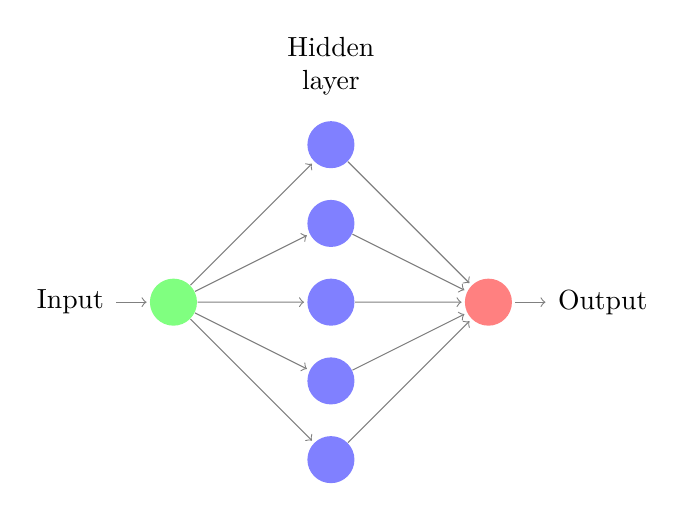
\begin{tikzpicture}[shorten >=1pt,->,draw=black!50, node distance=\layersep]
    \tikzstyle{every pin edge}=[<-,shorten <=1pt];
    \tikzstyle{neuron}=[circle,fill=black!25,minimum size=17pt,inner sep=0pt];
    \tikzstyle{input neuron}=[neuron, fill=green!50];
    \tikzstyle{output neuron}=[neuron, fill=red!50];
    \tikzstyle{hidden neuron}=[neuron, fill=blue!50];
    \tikzstyle{annot} = [text width=4em, text centered];
    \tikzmath{
      \nhidden = 5;
      \layersep = 2;
    }

    % Draw the input layer node
    \node[input neuron, pin=left:Input] (I) at (0,-\nhidden/2) {};

    % Draw the hidden layer nodes
    \foreach \name / \y in {1,...,\nhidden}
    \path[yshift=0.5cm]
    node[hidden neuron] (H-\name) at (\layersep,-\y cm) {};

    % Draw the output layer node
    \node[output neuron,pin={[pin edge={->}]right:Output}] (O) at (2*\layersep, -\nhidden/2) {};

    % Connect every node in the input layer with every node in the
    % hidden layer.
    \foreach \dest in {1,...,\nhidden}
    \path (I) edge (H-\dest);

    % Connect every node in the hidden layer with the output layer
    \foreach \source in {1,...,\nhidden}
    \path (H-\source) edge (O);

    % Annotate the layers
    \node[annot,above of=H-1, node distance=1cm] (hl) {Hidden layer};
  \end{tikzpicture}
  \caption{An illustration of the type of artificial neural network used for regression. Note our model was constructed with 15 nodes in the hidden layer.}
  \label{fig:ANN}
\end{figure}

One aspect to keep in mind when designing a neural network is to limit the number of trainable parameters and the number of training epochs in order to prevent overfitting.
However, in our case we have so many data points in our training data, and so densely distributed in the domain $[0, 15]$ of wind speed, that we were never able to overfit the model.
Indeed, we can inspect visually in \cref{fig:q1-prediction-plots} that the neural network is not overfitted: it results in a ``smooth'' function, not jagged.


\subsection*{Results}

The RMSEs of all the different approaches are summarised as follows:
\begin{center}
  \csvautobooktabular{data/q1_RMSE.csv}
\end{center}

See \cref{fig:q1-prediction-plots} for plots of the 4 different predictions for $f$ on the testing data for November, compared wit the actual data.

\begin{figure}
  \centering
  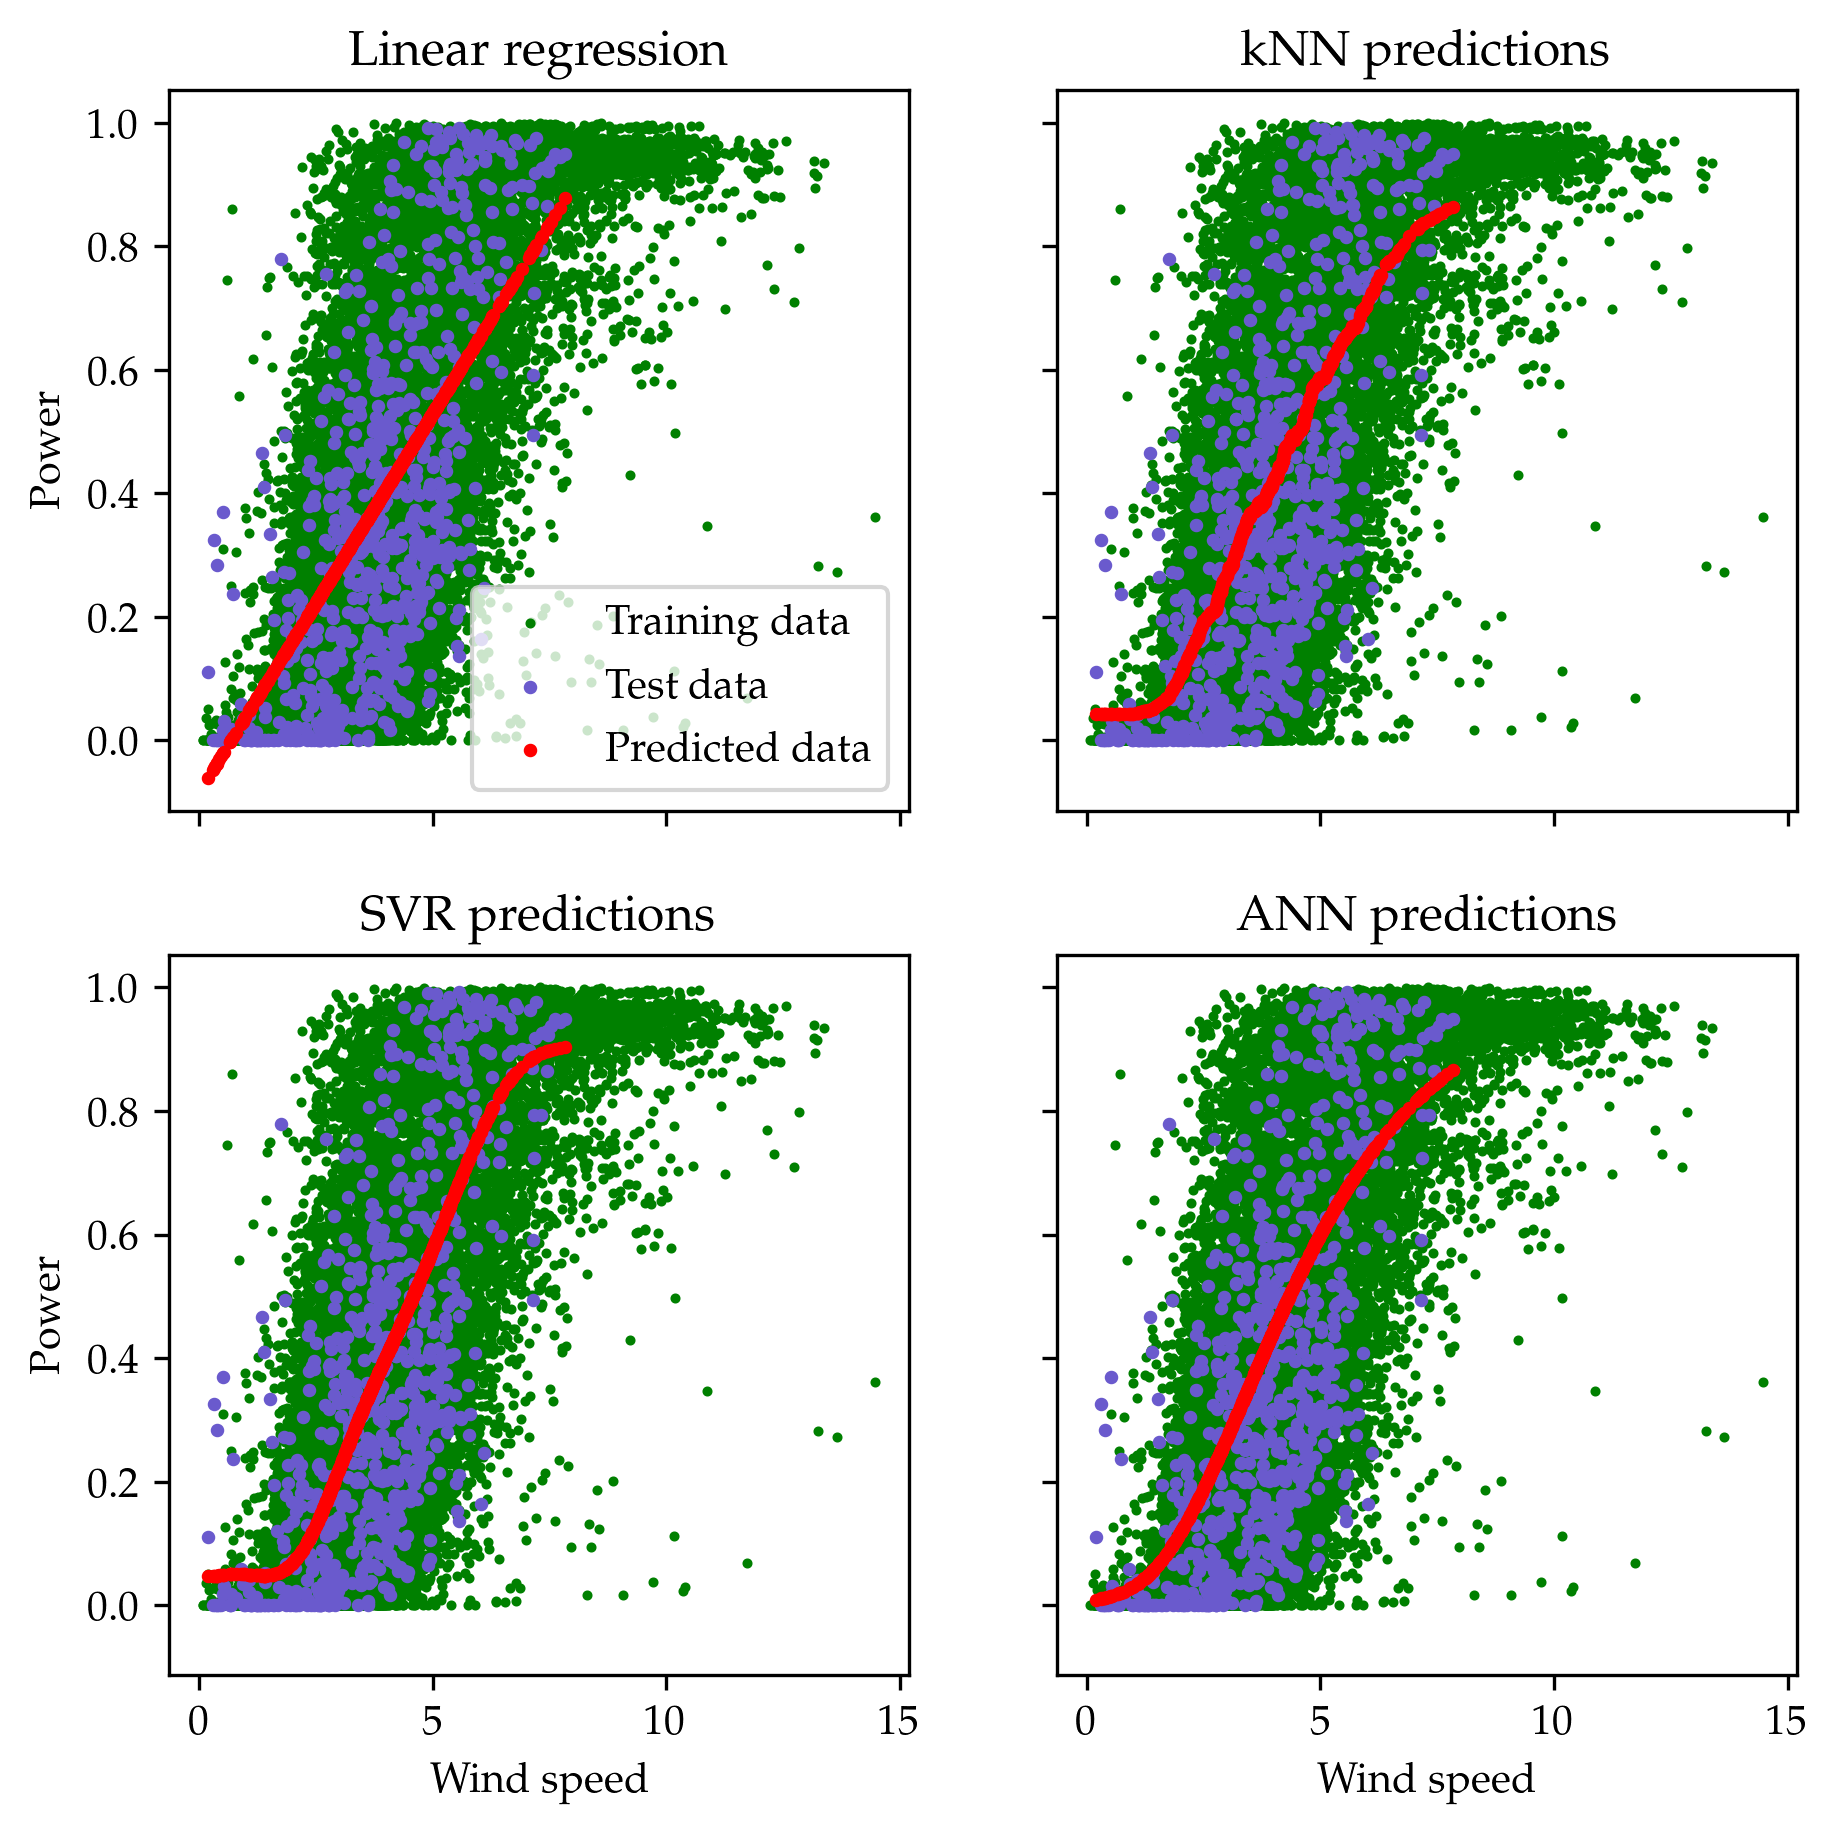
\includegraphics{figures/q1_prediction_plots.png}
  \caption{Plots of the various predictions for $f$ against the training and test data.}
  \label{fig:q1-prediction-plots}
\end{figure}

Moreover, see \cref{fig:q1-forecast-plots} for the power output forecasts for November by the different machine learning models, plotted over time.

\begin{figure}
  \centering
  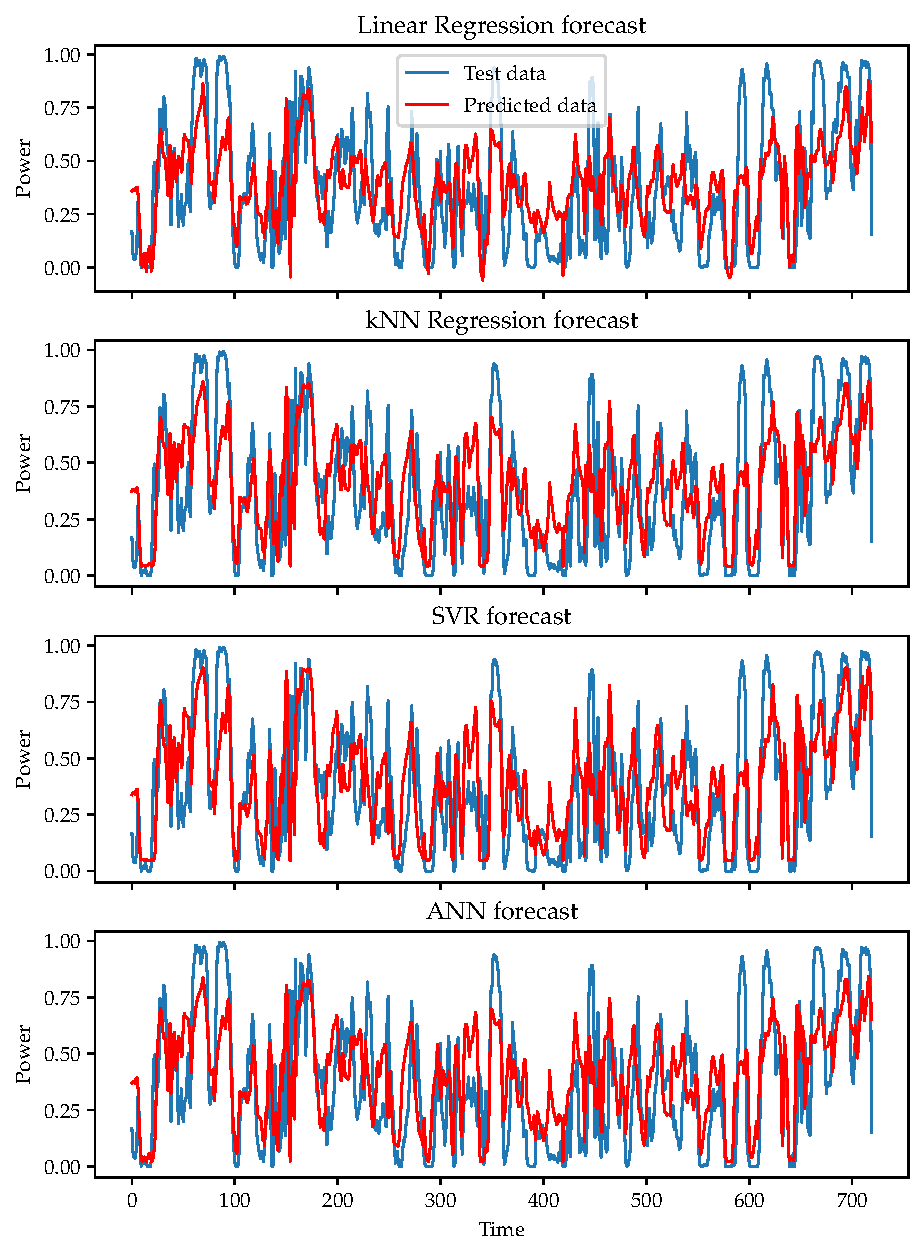
\includegraphics{figures/q1_forecast_plots}
  \caption{Plots of the forecast power output in November 2013 for different machine learning models.}
  \label{fig:q1-forecast-plots}
\end{figure}


\subsection*{Discussion}

In terms of RMSE, all the models perform similarly.
Visually, it looks like the kNN, SVR and ANN models all fit the data a little better than linear regression, with small differences between the three more advanced models especially towards the tails of the data.
It may be noted that linear regression gives \emph{negative} power outputs for very low wind speeds; not a particularly realistic outcome.

\subsubsection*{Accuracy of the results}

One surprising outcome in this question is the apparent adequacy of linear regression.
We can see in~\cref{fig:q1-prediction-plots} that the relationship between wind speed and power output does not appear to be quite linear, so we would expect more sophisticated models to perform significantly better than linear regression.
Instead, the RMSE for linear regression is around the same as for the other models.
What has happened?

It is revealing to investigate the RMSEs between predictions and actual power output for the period 01.01.2012--31.10.2013, which we have used as training data.
Evaluating models on the training data is not always a good idea, mainly because over-fitting models will appear to have a very low error which doesn't reflect their predicting accuracy.
However, in our case we can see in \cref{fig:q1-prediction-plots} that none of our models have over-fitted the training data.\footnote{An over-fitted prediction would look like a ``jagged'' red line following individual points.}
This makes sense, because we have more than 16000 measurements for a single parameter to train on: it would be exceedingly difficult for models to over-fit this data.

With all that said, consider the RMSEs of the four machine learning models on the training data:
\begin{center}
  \csvautobooktabular{data/q1_RMSE_training.csv}
\end{center}

As we can see, all the more advanced models outperform linear regression here, with $k$-nearest-neighbour regression and the artificial neural network model performing the best.
We can conclude that these models have indeed found a better fit to the training data than linear regression.
This affirms our observation that the relationship between wind speed and power output is not quite linear.

So why does linear regression perform better on the testing data (November 2013)?
The data for November 2013 differs from the average for 2012--2013, and we conclude that the relationship between wind speed and power output happened to be more linear in November 2013 than during the rest of 2012--2013.
This explains the ``unexpectedly'' good performance of the linear regression model for November 2013.

Indeed, it is not unusual for weather conditions to deviate significantly from the average for a duration of a month.
We strongly suspect that if we tested the machine learning models on data covering a longer period (e.g.\ 2014--2015), we would see a similar performance as on the testing data, with the $k$-nearest-neighbour and neural network models outperforming linear regression in prediction accuracy.


\subsubsection*{Remark on neural network design complexity}

Finally, we note that we tried out a number of alternative, more complex neural network designs, but none improved significantly on the final simple design.
In particular, we experimented with multi-layer networks such as a network with two hidden layers consisting of 32 nodes each or even with four hidden layers containing 32, 64, 32 and 16 nodes respectively.
(For these models, we use a rectified linear activation function.)
However, out findings suggest that the function $f$ to be learned is simple enough that a single-layer neural network already achieves the best possible result.

This is unsurprising, since $f$ is a 1-dimensional function that seems very smooth on its domain.
Indeed, a quick test shows that a degree 3 polynomial fits the training data with a RMSE of \input{data/q1_RMSE_poly_training.txt}; about as good as any of the other models.
This shows that the power output function can be accurately described by only 4 real numbers.


\clearpage




\subsection*{Discussion}

Linear regression again was not outperformed significantly by more advanced models such as SVR and ANN (even a complex ANN design).
This was seen at both a window size of 4 and 20.
This initially suggests that the power output function $p_t = f(p_{t-k}, \dots, p_{t-1})$ has a relatively simple shape, and is not hard to predict.
The fact that the RMSE is still significant can be explained by unforeseen changes in weather which are impossible to predict using solely historical power output.

These conclusions are drawn in doubt by the surprisingly good performance of the RNN model.
In the results section above, we see that the RMSE achieved by the RNN model is more than 5-6 times better than the errors achieved by the other models.
Moreover, the extrodinarily good performance seems to be entire due to the use of a bidirectional LSTM approach.
Without the use of a bidirectional layer, the performance of the RNN model is more similar but still slightly better compared to MLR, SVR and ANN.

This suggests that there may be patterns to the time series that cannot be captured by more conventional models but that are captured very well by a bidirectional recurrent neural network.
These significant patterns are presumably related to time-reversal effects, considering the nature of bidirectional RNNs. We know that over long sequences, we have the problem of the gradient being washed out during training, and this also applies to the LSTM at some point. Taking this into account, we think that the bidirectional computation of the sequence starting at both $t = 0$ and $t = n$ (reverse order) is beneficial during the learning process due to the length of the sequence and the importance of different time-steps and how much it can learn from each time-step. The most important time-step is the time-step that is closest ($t = n-1$) to the ``current'' time-step $t = n$. One could be confident assuming that the gradient is not washed out at $t = n-1$ when considering the sequence $t = n, n-1, \dots, 0$. However, exactly why bidirectional RNNs perform so much better than other models, and for what kind of data this holds, are questions that would be interesting to investigate further.


\printbibliography


\end{document}


% Local Variables:
% TeX-engine: xetex
% End: